\justifying
Σε αυτό το κεφάλαιο, θα υλοποιηθούν οι αλγόριθμοι που αναφέρθηκαν προηγουμένως, δηλαδή ο \en FastICA, \gr ο π\en CA \gr και ο \en AMUSE. \gr Συγκεκριμένα, θεωρούμε τα πηγαία σήματα \en $\mathbf{S} \in \mathbb{R}^{n \times m}$ \gr, όπου \en $n$ \gr ο αριθμός των σημάτων και \en $m$ \gr ο αριθμός των δειγμάτων, είτε αμιγώς περιοδικά (ημίτονα, τετραγωνικούς παλμούς, κλπ.) είτε περίπλοκα σήματα με μεταβλητή περιοδικότητα, δηλαδή αφού σχηματιστούν, επαναλαμβάνονται στο πεδίο του χρόνου ώστε να συμπληρώσουν την καθορισμένη διάρκεια, είτε πραγματικά βιοσήματα που έχουμε λάβει από αισθητήρες.
\\[0.5 \baselineskip]
Υποθέτουμε ότι τα σήματα ως προς εκτίμηση \en $\mathbf{X} \in \mathbb{R}^{n \timeσ m}$ \gr, σύμφωνα με το μοντέλο \en BSS, \gr είναι:
\begin{align*}
    \mathbf{X} = \mathbf{B} \mathbf{S} + \mathbf{N} \quad \mathbf{X} \in \mathbb{R}^{n \times m}
\end{align*}
όπου \en $\mathbf{B} \in \mathbb{R}^{n \times n}$ \gr ο πίνακας μίξης και \en $\mathbf{N} \in \mathbb{R}^{n \times m}$ \gr ο πίνακας προσθετικού θορύβου που ακολουθεί την κατανομή \en $\mathcal{N} \sim (0,\sigma)$. \gr
\\[0.5 \baselineskip]
Ο σκοπός είναι να βρεθεί ένας πίνακας που θα μετασχηματίζει τα μιξαρισμένα σήματα σε έναν πίνακα \en $\mathbf{\hat{S}} = \mathbf{W} \mathbf{X}$ \gr που θα είναι όσο πιο κοντά γίνεται στα πηγαία σήματα \en $\mathbf{S}$. \gr
\section{Τεχνητά Σήματα}
\justifying
Για την αξιολόγηση των αλγορίθμων θα χρησιμοποιηθεί το παρακάτω κριτήριο\cite{pi:17}: \en
\begin{align} \label{eq:5.1.1}
J( \mathbf{P} ) = \frac{\parallel \mathbf{P} - diag(\mathbf{P}) \parallel ^2} { \parallel \mathbf{P} \parallel ^2}
\end{align} \gr
όπου \en $\mathbf{P} = \mathbf{W} \mathbf{A} , \mathbf{P} \in \mathbb{R}^{n \times n}$ \gr και \en $\parallel . \parallel $ \gr η ευκλείδια νόρμα. Το κριτήριο \eqref{eq:5.1.1} είναι μη αρνητικό και ισούται με το μηδέν όταν \en $\mathbf{W} =  \mathbf{A}^{-1}$ \gr, δηλαδή όταν ο πίνακας \en $\mathbf{P}$ \gr είναι πίνακας αντιμετάθεσης. Οι αλγόριθμοι λειτουργούν ικανοποιητικά όταν η \eqref{eq:5.1.1} είναι κοντά στο μηδέν. 
\newpage
\noindent Το παραπάνω κριτήριο θα τροποποιηθεί λίγο ώστε να αντιμετωπίσει την αδυναμίες της μεθόδου \en FastICA \gr ως προς την λανθασμένη σειρά των ανεξάρτητων συνιστωσών. Για αυτό, θα πρέπει να μετατραπεί ο πίνακας \en $\mathbf{P}$ \gr σε έναν πιο "διαγώνιο", βρίσκοντας την θέση του μεγαλύτερου στοιχείου κάθε σειράς και με βάση αυτό να αλλαχθεί η σειρά των γραμμών του πίνακα $\mathbf{P}$. Mε την παραπάνω μετατροπή αλλάζει μόνο η σειρά των ανεξάρτητων συνιστωσών και όχι οι ίδιες συνιστώσες.
\subsection{Περιοδικά Σήματα}
\justifying
Θεωρούμε ως σήματα πηγών: \en
\begin{align*}
    &s_1 = square(\frac{2\pi}{T_1} t) \\
    &s_2 = \sin (\frac{2\pi}{T_2} t) \\
    &s_3 = sawtooth(\frac{2\pi}{T_3} t)
\end{align*} \gr
μαζί με προσθήκη 'λευκού' θορύβου.
\\
O πίνακας πίνακα μίξης: \en
\begin{align*}
    \mathbf{A} = \begin{bmatrix}
    -0.581432 & -2.96086 & 1.23499 \\
    -0.878361 & 0.25808 & 1.52502 \\
    1.20338 & 0.891327 & 0.918677
    \end{bmatrix}  \quad det(\mathbf{A}) = -8.52
\end{align*} \gr
Οι περίοδοι των σημάτων των πηγών είναι \en $T_1 = 0.11 s$, $T_2 = 0.25 s$ \gr και \en $T_3 = 0.47 s$. \gr Η διάρκεια των σημάτων είναι 5 δευτερόλεπτα ενώ η συχνότητα δειγματοληψίας είναι \en $f_s = 500 Hz$. \gr Τα σήματα πηγών με την προσθήκη θορύβου και τα πεπλεγμένα σήματα φαίνονται στις εικόνες \ref{fig:5.1a} και \ref{fig:5.1b}.
\begin{figure}[H]
    \centering
    \begin{subfigure}{0.48 \textwidth}
        \centering
       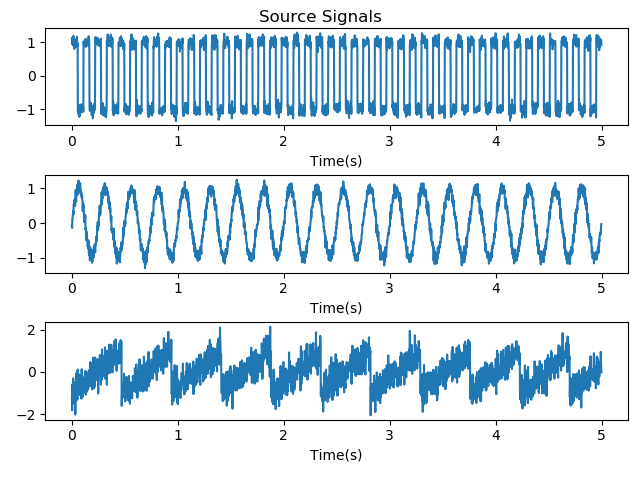
\includegraphics[width=\textwidth]{fwto/Signals_ica_1.png} \en
        \caption{} \gr
        \label{fig:5.1a}
    \end{subfigure}%
    \hfill
    \begin{subfigure}{0.48 \textwidth}
        \centering
       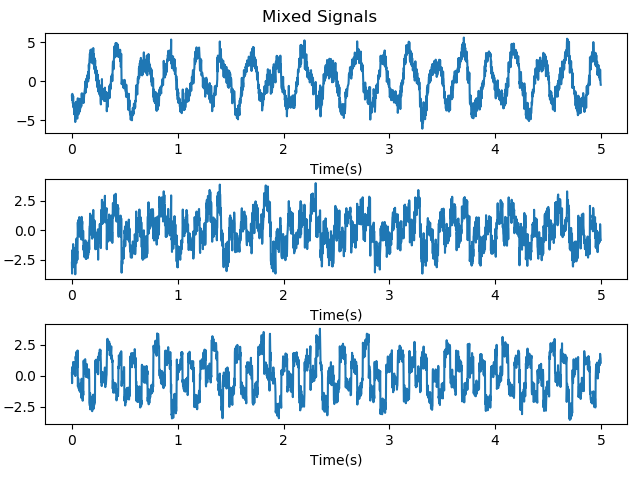
\includegraphics[width=\textwidth]{fwto/Mixed_ica_1.png}
        \en
        \caption{} \gr
        \label{fig:5.1b}
    \end{subfigure}%
    \gr
    \caption{Περιοδικές Πηγές και Μιξαρισμένα Σήματα}
\end{figure}
\noindent Τα σχήματα \en \ref{fig:5.2a} \gr και \en \ref{fig:5.2b} \gr είναι οι ανεξάρτητες συνιστώσες που εξάγει ο αλγόριθμος \en FastICA \gr για \en 'logcosh' \gr, τα σχήματα \en \ref{fig:5.3a} \gr   και \en \ref{fig:5.3b} \gr  για \en 'exp' \gr και τα σχήματα \en \ref{fig:5.4a} \gr και \en \ref{fig:5.4b} \gr για \en 'cube' \gr.
\begin{figure}[H]
    \centering
    \begin{subfigure}{0.48 \textwidth}
        \centering
        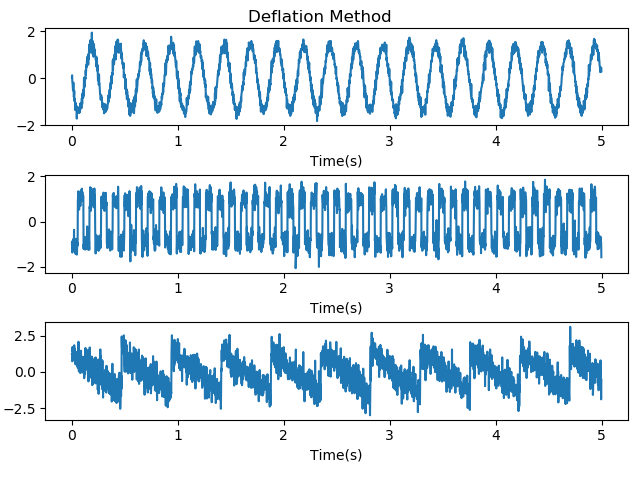
\includegraphics[width=\textwidth]{fwto/defla_ica_1_logcosh.png} \en
        \caption{Deflation} \gr
        \label{fig:5.2a}
    \end{subfigure}%
    \hfill
    \begin{subfigure}{0.48 \textwidth}
        \centering
    `   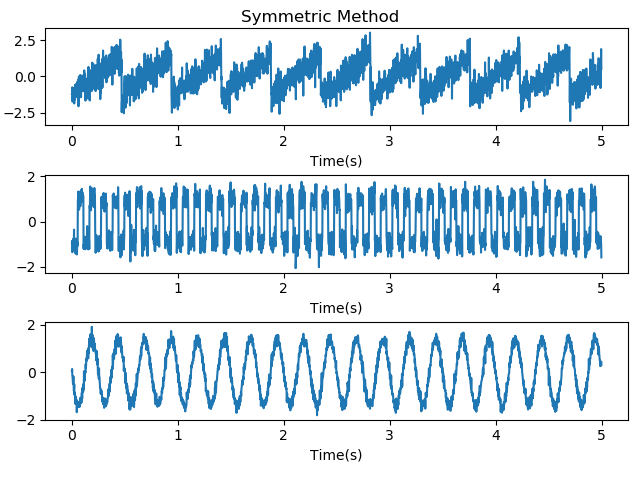
\includegraphics[width=\textwidth]{fwto/Symmetric_ica_1_logcosh.png}
        \en
        \caption{Symmetric} \gr
        \label{fig:5.2b}
    \end{subfigure}%
    \gr
    \caption{Ανεξάρτητες Συνιστώσες περιοδικών σημάτων για \en g = 'logcosh' \gr}
\end{figure}
\begin{figure}[H]
    \centering
    \begin{subfigure}{0.48 \textwidth}
        \centering
       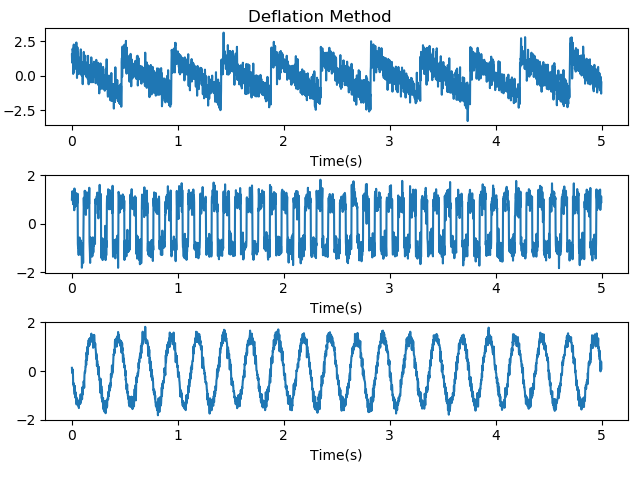
\includegraphics[width=\textwidth]{fwto/defla_ica_1_exp.png} \en
        \caption{Deflation} \gr
        \label{fig:5.3a}
    \end{subfigure}%
    \hfill
    \begin{subfigure}{0.48 \textwidth}
        \centering
       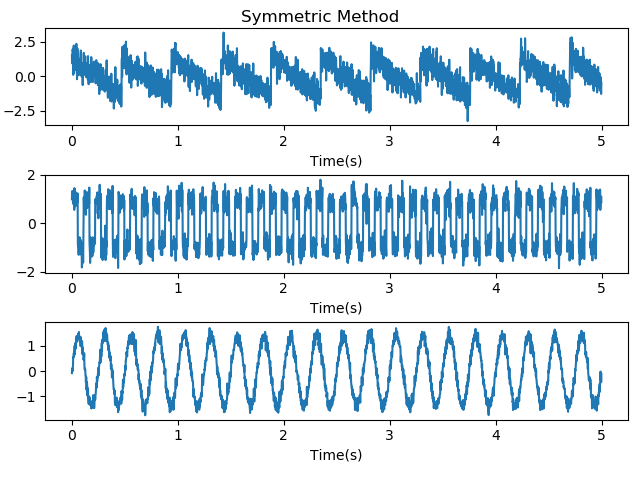
\includegraphics[width=\textwidth]{fwto/Symmetric_ica_1_exp.png}
        \en
        \caption{Symmetric} \gr
        \label{fig:5.3b}
    \end{subfigure}%
    \gr
    \caption{Ανεξάρτητες Συνιστώσες περιοδικών σημάτων για \en g = 'exp' \gr}
\end{figure}
\begin{figure}[H]
    \centering
    \begin{subfigure}{0.48 \textwidth}
        \centering
       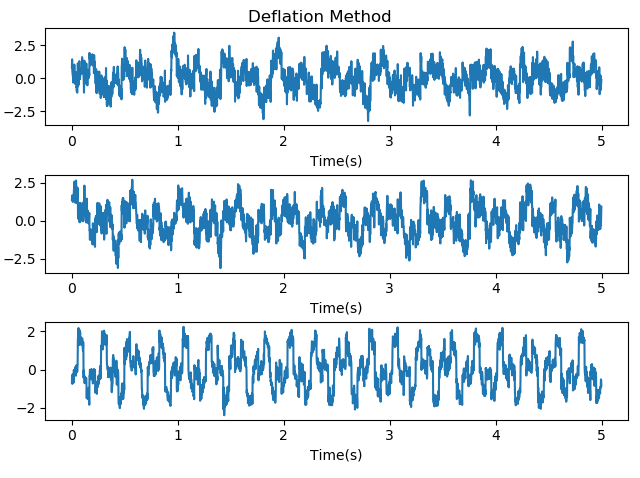
\includegraphics[width=\textwidth]{fwto/Deflation_ica_1_cube.png}\en
        \caption{Deflation} \gr
        \label{fig:5.4a}
    \end{subfigure}%
    %\hfill
    \begin{subfigure}{0.48 \textwidth}
        \centering
       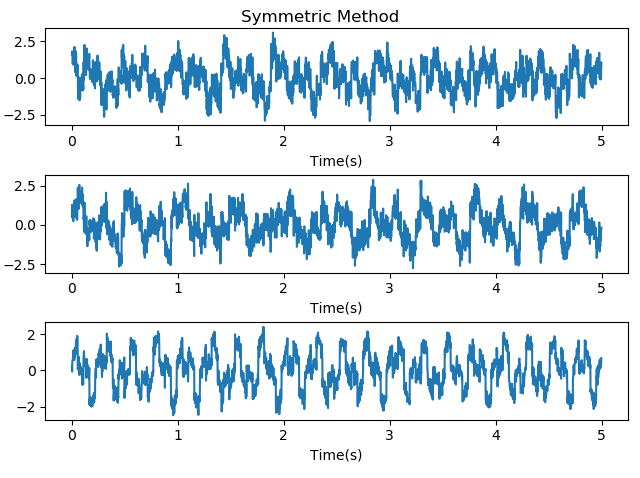
\includegraphics[width=\textwidth]{fwto/Symmetric_ica_1_cube.png}
        \en
        \caption{Symmetric} \gr
        \label{fig:5.4b}
    \end{subfigure}%
    \gr
    \caption{Ανεξάρτητες Συνιστώσες περιοδικών σημάτων για \en g = 'cube' \gr}
\end{figure}
\noindent Στα σχήματα \en \ref{fig:5.5a} \gr και \en \ref{fig:5.5b} \gr φαίνονται οι περιοδικές συνιστώσες που εξάγουν οι αλγόριθμοι π\en CA \gr και \en AMUSE \gr, ενώ στα σχήματα \en \ref{fig:5.6a} \gr και \en \ref{fig:5.6b} \gr τα αντίστοιχα περιοδικά σφάλματα.
\begin{figure}[H]
    \centering
    \begin{subfigure}{0.48 \textwidth}
        \centering
       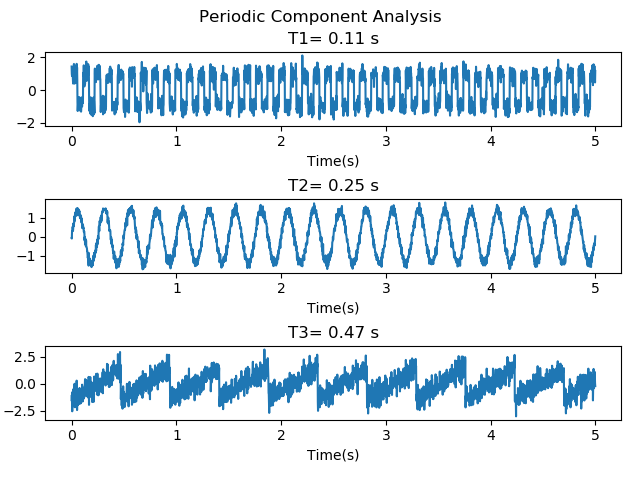
\includegraphics[width=\textwidth]{fwto/piCA_1.png}\en
        \caption{\gr Κανονική \en \pi CA} \gr
        \label{fig:5.5a}
    \end{subfigure}
    \hfill
    \begin{subfigure}{0.48 \textwidth}
        \centering
       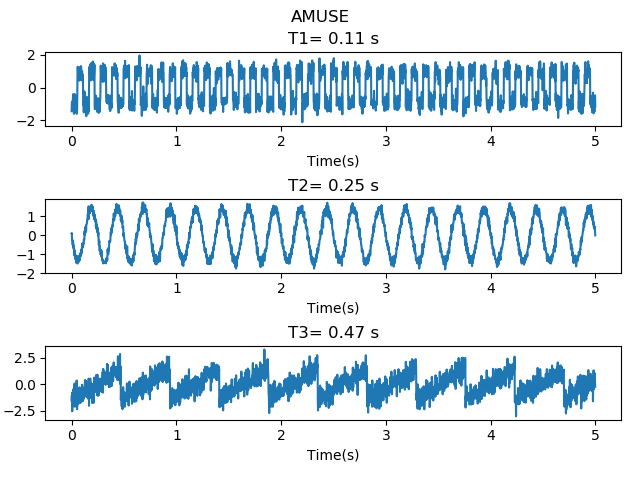
\includegraphics[width=\textwidth]{fwto/Amuse_1.png}
        \en
        \caption{AMUSE} \gr
        \label{fig:5.5b}
    \end{subfigure}
    \gr
    \caption{Εξαγωγή Περιοδικών Συνιστωσών για \en $T_1 = 0.11$ s, $T_2 = 0.25$ s \gr και \en $T_3 = 0.47$ s \gr}
\end{figure}
\begin{figure}[H]
    \centering
    \begin{subfigure}{0.48 \textwidth}
        \centering
       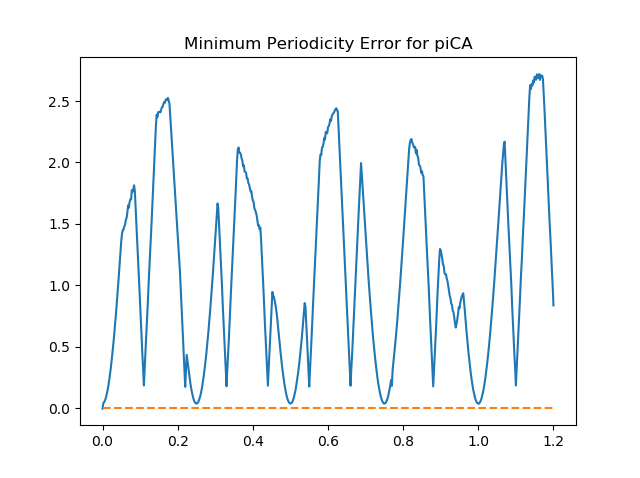
\includegraphics[width=\textwidth]{fwto/piCA_Error_1.png}\en
        \caption{\gr Κανονική \en \pi CA} \gr
        \label{fig:5.6a}
    \end{subfigure}
    \hfill
    \begin{subfigure}{0.48 \textwidth}
        \centering
       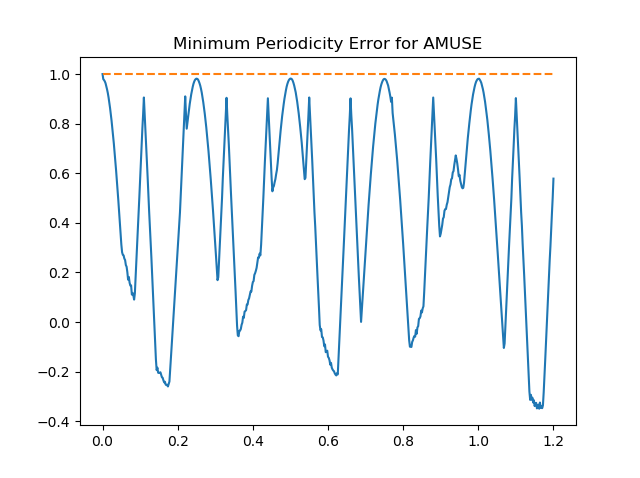
\includegraphics[width=\textwidth]{fwto/Amuse_Error_1.png}
        \en
        \caption{AMUSE} \gr
        \label{fig:5.6b}
    \end{subfigure}
    \gr
    \caption{Τα ελάχιστα σφάλματα για χρονική καθυστέρηση από 0 έως 1.2 δευτερόλεπτα}
\end{figure}
\noindent Τέλος, οι συντελεστές απόδοσης που υπολογίζονται από την \eqref{eq:5.1.1} φαίνονται παρακάτω: \en
\begin{table}[H] 
\centering
\begin{tabular}{|c|c|l|} 
\hline
          & Deflational  & Symmetric  \\ \hline
'logcosh' & 0.000847636 &  0.000818582 \\ \hline
'exp'     & 0.000951913 &  0.000261241 \\ \hline
'cube'    & 0.630938755 &  0.663469048 \\ \hline
πCA       & \multicolumn{2}{c|}{6.16798765e-05} \\ \hline
AMUSE     & \multicolumn{2}{c|}{6.16798765e-05} \\ \hline
\end{tabular}
\gr
\caption{Κριτήριο απόδοσης για κάθε υλοποιήσιμη μέθοδο}
\label{table:5.1}
\end{table}
\noindent Όπως βλέπουμε από τις γραφικές παραστάσεις, παρατηρούμε ότι, παρόλο της παρουσίας προσθετικού θορύβου, και η μέθοδος \en FastICA \gr αλλά και η π\en CA \gr αναγνωρίζουν πλήρως τα σήματα, εκτός της περίπτωσης \en 'cube' \gr της \en FastICA \gr . Από τον πίνακα απόδοσης \ref{table:5.1}, παρατηρούμε ότι σχεδόν όλοι οι αλγόριθμοι έχουν τιμή περίπου ίση με το 0, άρα προσεγγίζουν έναν πίνακα αντιμετάθεσης και επίσης, οι αλγόριθμοι που υποθέτουν περιοδικότητα έχουν αμυδρά καλύτερα αποτελέσματα κάτι που είναι προφανές εφόσον τα σήματα πηγών που χρησιμοποιήσαμε είναι περιοδικά.
\subsection{Ψευδό-Περιοδικά Σήματα}
\justifying
Θεωρούμε ως σήματα πηγών τα σήματα που φαίνονται στο σχήμα \ref{fig:5.7a}.
Βλέπουμε ότι τα δυο πρώτα σήματα αποτελούν συνδυασμούς σημάτων τα οποία έχουν επαναληφθεί στο πεδίο του χρόνου, κάνοντας τα ψευδό-περιοδικά ενώ το τελευταίο σήμα αποτελείται από 'λευκό' θόρυβο. Επιπλέον, για τα περιοδικά σήματα, οι περίοδοι επιλέχθηκαν αρχικά ως \en $T_1 = 0.5$ s \gr και \en $T_2 = 0.754$ s \gr και μεταβάλλουμε των αριθμό δειγμάτων τους κατά $a , b \in [-100 , 100]$ αντίστοιχα, οπότε δεν γνωρίζουμε την εκάστοτε περίοδο ακριβώς.
\\
Η διάρκεια των σημάτων είναι 5 δευτερόλεπτα ενώ η συχνότητα δειγματοληψίας είναι \en $f_s = 1 KHz$.\gr 
\\
Ο πίνακας μίξης είναι: \en
\begin{align*}
    \mathbf{A} = \begin{bmatrix}
    0.00740553 &  1.05634461 & -0.52022631 \\
    -0.00531442 &  0.95287344 & -0.26333002 \\
    -2.39713001 & -0.52477855 & -0.67513928 
    \end{bmatrix} \quad det(\mathbf{A}) = -0.5325
\end{align*}
\gr 
Τα σήματα πηγών και τα πεπλεγμένα σήματα φαίνονται στις εικόνες \en \ref{fig:5.7a} \gr και \en \ref{fig:5.7b} \gr.
\begin{figure}[H]
    \centering
    \begin{subfigure}{0.48 \textwidth}
        \centering
       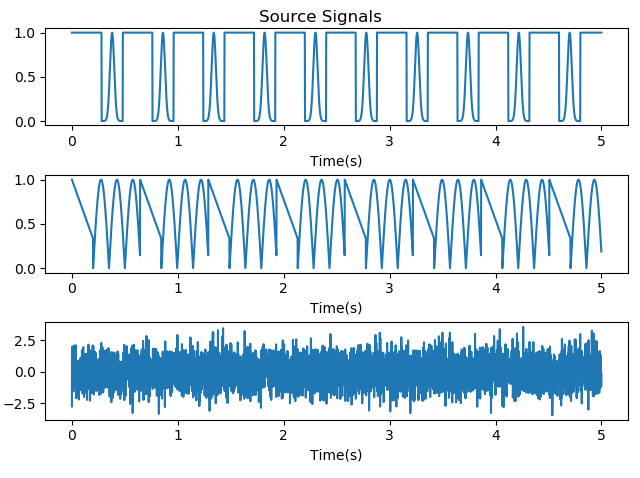
\includegraphics[width=\textwidth]{fwto/source.png} \en
        \caption{} \gr
        \label{fig:5.7a}
    \end{subfigure}
    \hfill
    \begin{subfigure}{0.48 \textwidth}
        \centering
       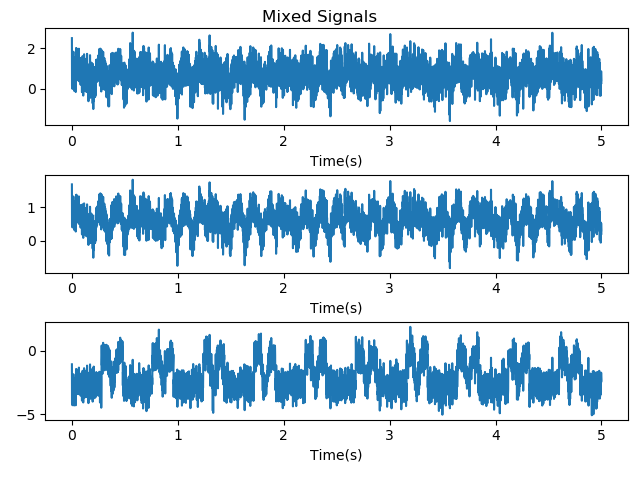
\includegraphics[width=\textwidth]{fwto/mixed.png}
        \en
        \caption{} \gr
        \label{fig:5.7b}
    \end{subfigure}
    \gr
    \caption{Ψευδο-περιοδικές Πηγές και Μιξαρισμένα Σήματα}
\end{figure}
\noindent Τα σχήματα \en \ref{fig:5.8a} \gr και \en \ref{fig:5.8b} \gr είναι οι ανεξάρτητες συνιστώσες που εξάγει ο αλγόριθμος \en FastICA \gr για \en 'logcosh' \gr, τα σχήματα \en \ref{fig:5.9a} \gr   και \en \ref{fig:5.9b} \gr  για \en 'exp' \gr και τα σχήματα \en \ref{fig:5.10a} \gr και \en \ref{fig:5.10b} \gr για \en 'cube' \gr.
\begin{figure}[H]
    \centering
    \begin{subfigure}{0.48 \textwidth}
        \centering
       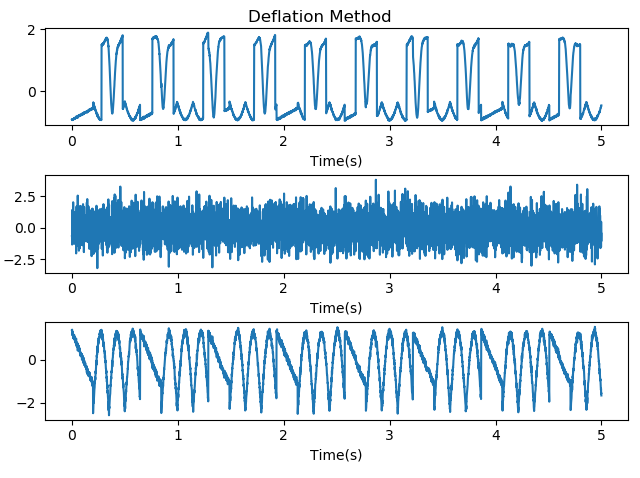
\includegraphics[width=\textwidth]{fwto/logcosh_def.png} \en
        \caption{Deflation} \gr
        \label{fig:5.8a}
    \end{subfigure}
    \hfill
    \begin{subfigure}{0.48 \textwidth}
        \centering
       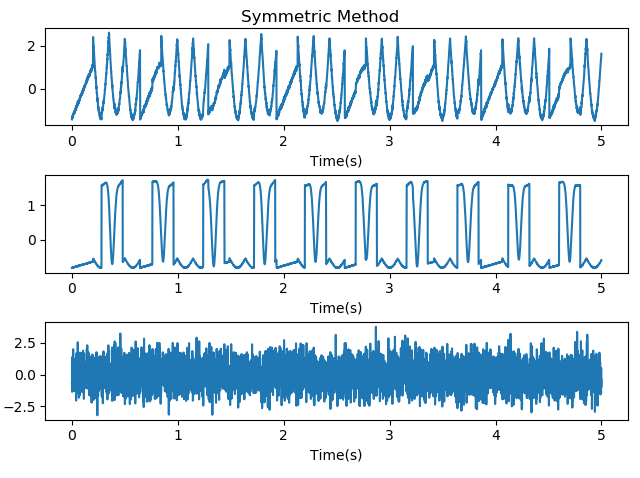
\includegraphics[width=\textwidth]{fwto/logcosh_sym.png} \en
        \en
        \caption{Symmetric} \gr
        \label{fig:5.8b}
    \end{subfigure}
    \gr
    \caption{Ανεξάρτητες Συνιστώσες περιοδικών σημάτων για \en g = 'logcosh' \gr}
\end{figure}
\begin{figure}[H]
    \centering
    \begin{subfigure}{0.48 \textwidth}
        \centering
       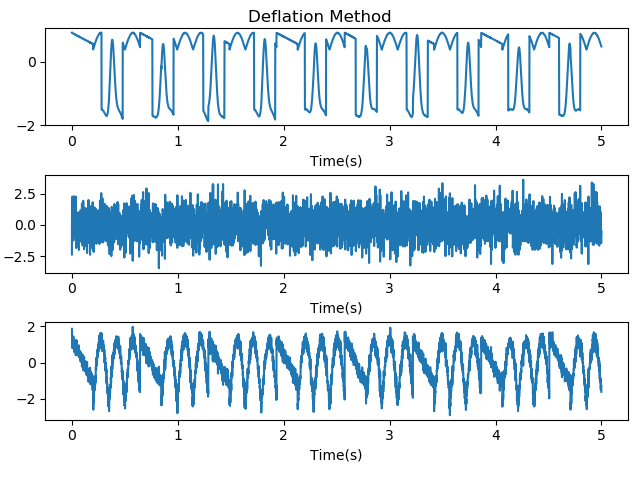
\includegraphics[width=\textwidth]{fwto/exp_def.png} \en
        \caption{Deflation} \gr
        \label{fig:5.9a}
    \end{subfigure}
    \hfill
    \begin{subfigure}{0.48 \textwidth}
        \centering
       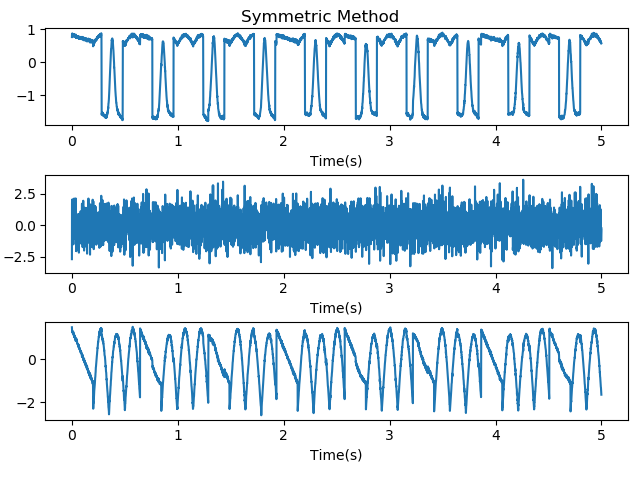
\includegraphics[width=\textwidth]{fwto/exp_sym.png}
        \en
        \caption{Symmetric} \gr
        \label{fig:5.9b}
    \end{subfigure}
    \gr
    \caption{Ανεξάρτητες Συνιστώσες περιοδικών σημάτων για \en g = 'exp' \gr}
\end{figure}
\begin{figure}[H]
    \centering
    \begin{subfigure}{0.48 \textwidth}
        \centering
       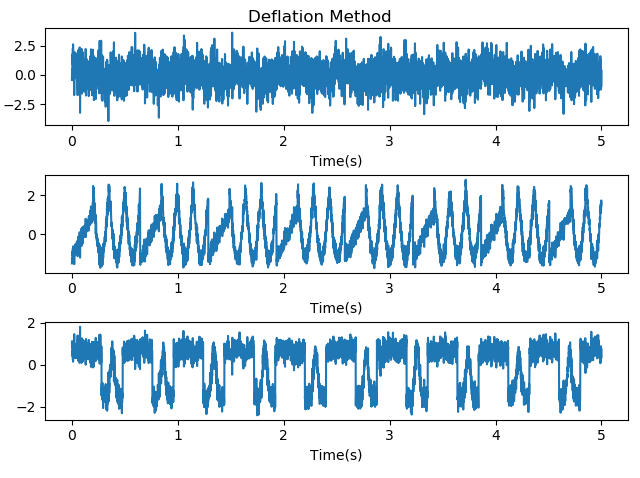
\includegraphics[width=\textwidth]{fwto/cube_def.png}\en
        \caption{Deflation} \gr
        \label{fig:5.10a}
    \end{subfigure}
    \hfill
    \begin{subfigure}{0.48 \textwidth}
        \centering
       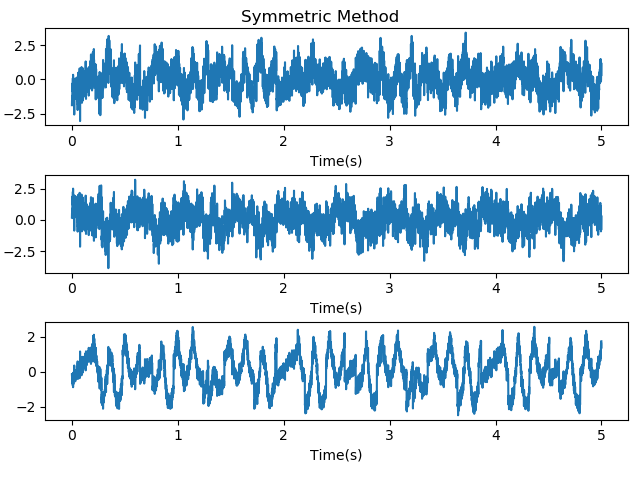
\includegraphics[width=\textwidth]{fwto/cube_sym.png}
        \en
        \caption{Symmetric} \gr
        \label{fig:5.10b}
    \end{subfigure}
    \gr
    \caption{Ανεξάρτητες Συνιστώσες περιοδικών σημάτων για \en g = 'cube' \gr}
\end{figure}
% fix ref
\noindent Στα σχήματα \en \ref{fig:5.11a} \gr και \en \ref{fig:5.11b} \gr φαίνονται οι περιοδικές συνιστώσες που εξάγουν οι αλγόριθμοι π\en CA \gr και \en AMUSE \gr, ενώ στα σχήματα \en \ref{fig:5.12a} \gr και \en \ref{fig:5.12b} \gr τα αντίστοιχα περιοδικά σφάλματα.
\en
\begin{figure}[H]
    \centering
    \begin{subfigure}{0.48 \textwidth}
        \centering
       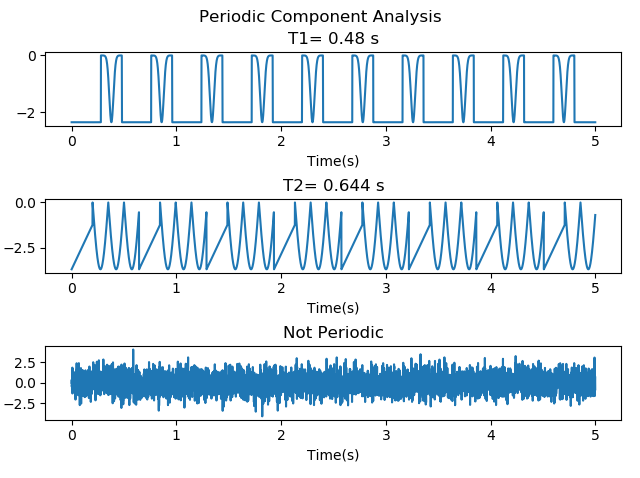
\includegraphics[width=\textwidth]{fwto/pica.png}\en
        \caption{\gr Κανονική \en \pi CA} \gr
        \label{fig:5.11a}
    \end{subfigure}
    \hfill
    \begin{subfigure}{0.48 \textwidth}
        \centering
       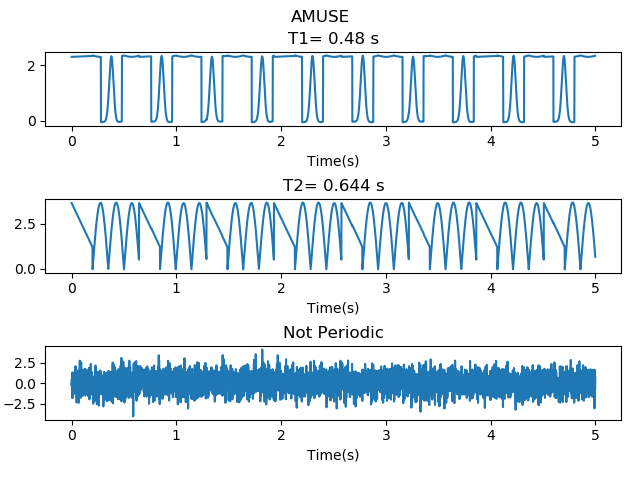
\includegraphics[width=\textwidth]{fwto/amuse.png}
        \en
        \caption{AMUSE} \gr
        \label{fig:5.11b}
    \end{subfigure}
    \gr
    \caption{Εξαγωγή Περιοδικών Συνιστωσών για \en $T_1 = 0.48$ s \gr και \en $T_2 = 0.644$ s \gr}
\end{figure}
\begin{figure}[H]
    \centering
    \begin{subfigure}{0.48 \textwidth}
        \centering
       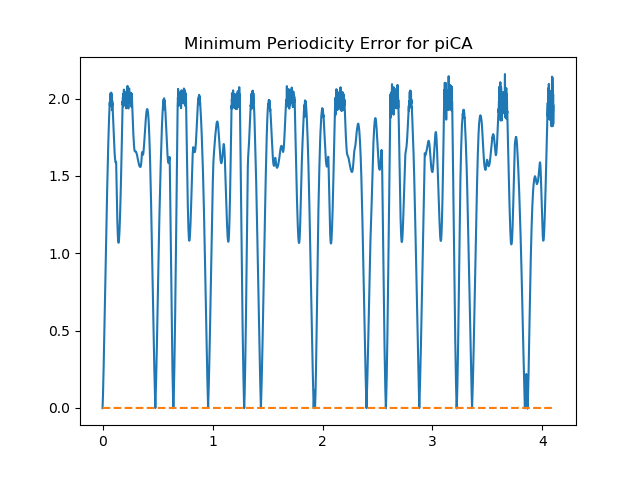
\includegraphics[width=\textwidth]{fwto/pica_error.png}\en
        \caption{\gr Κανονική \en \pi CA} \gr
        \label{fig:5.12a}
    \end{subfigure}
    \hfill
    \begin{subfigure}{0.48 \textwidth}
        \centering
       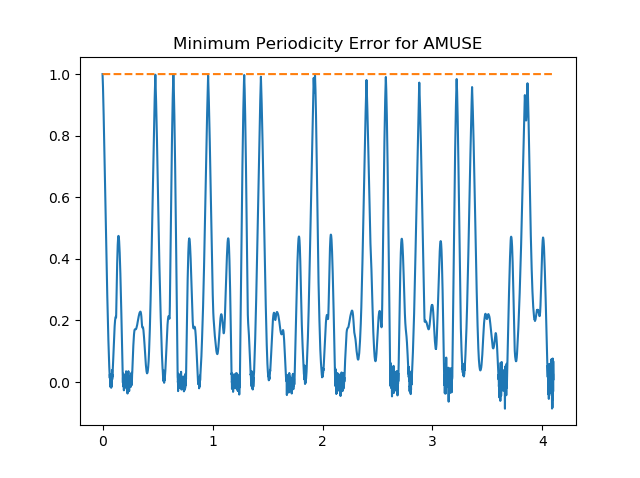
\includegraphics[width=\textwidth]{fwto/Amuse_Error.png}
        \en
        \caption{AMUSE} \gr
        \label{fig:5.12b}
    \end{subfigure}
    \gr
    \caption{Τα ελάχιστα σφάλματα για χρονική καθυστέρηση από 0 έως 4.2 δευτερόλεπτα}
\end{figure}
\noindent Τέλος, οι συντελεστές απόδοσης που υπολογίζονται από την \eqref{eq:5.1.1} φαίνονται παρακάτω: \en
\begin{table}[H] 
\centering
\begin{tabular}{|c|c|l|} 
\hline
          & Deflational  & Symmetric  \\ \hline
'logcosh' & 0.021798705 &  0.009850027 \\ \hline
'exp'     & 0.048388267 &  0.009237661 \\ \hline
'cube'    & 0.703621639 &  0.575454093 \\ \hline
πCA       & \multicolumn{2}{c|}{0.0005443894} \\ \hline
AMUSE     & \multicolumn{2}{c|}{0.0005443894} \\ \hline
\end{tabular}
\gr
\caption{Κριτήριο απόδοσης για κάθε υλοποιήσιμη μέθοδο}
\label{table:5.2}
\end{table}
\newpage
\noindent Παρατηρούμε ότι ο αλγόριθμος \en FastICA \gr και στις 3 περιπτώσεις, δεν εξάγει τα διάφορα σήματα επακριβώς αλλά εποπτικά, καθώς προσθέτει θόρυβο σε συνιστώσες που δεν είχαν, αντίθετα με τους αλγορίθμους π\en CA \gr και \en AMUSE \gr . Αυτό μπορεί να οφείλεται στο γεγονός ότι τα δεδομένα μας είναι αφιλτράριστα καθώς μπορεί να εμπεριέχονται συχνότητες στα δεδομένα μας που να δημιουργούν μια συσχέτιση με τον "λευκό" θόρυβο, κάνοντας τα μη-ανεξαρτήτα.
\section{Βιοσήματα}
\justifying
\iffalse
Κριτήριο αξιολόγησης μάλλον SNR na koitaxw papers
\fi
\subsection{Τεχνητά Βιοσήματα}
\justifying
Τα παρακάτω σήματα περιέχουν και πραγματικές και συνθετικές κυματομορφές, οι οποίες χρησιμοποιούνται για έλεγχο σε συσκευές που εποπτεύονται ηλεκτροκαρδιογραφήματα τα οποία λάβαμε από το \en Physionet ATM \gr \cite{signals:18} σε μορφή \en .txt \gr μέσω του πακέτου \en WFDB \gr \cite{db:19} από το \en Cygwin. \gr Επιλέγουμε 3 από τα διαθέσιμα σήματα, συγκεκριμένα τα \en "aami3a", "aami3b", \gr και \en "aami4a" \gr στα οποία δεν γνωρίζουμε την περίοδο τους. Καλούμαστε να αναγνωρίσουμε τα περιοδικά σημάτα, όπως και την περίοδο του καθενός, εκτελώντας τους αλγορίθμους με είσοδο των πίνακα που δημιουργείται από τα παραπάνω αρχεία. Το κάθε σήμα έχει διάρκεια 10 δευτερολέπτων και ρυθμό δειγματοληψίας ίσο με 720 \en Hz \gr, ανάλυση 12 \en bits \gr και τα πλάτος του κάθε σήματος είναι σε \en mV \gr. 
\\ [0.5 \baselineskip]
Τα σήματα πηγής φαίνονται στο σχήμα \ref{fig:5.13}:
\begin{figure}[H]
    \centering
    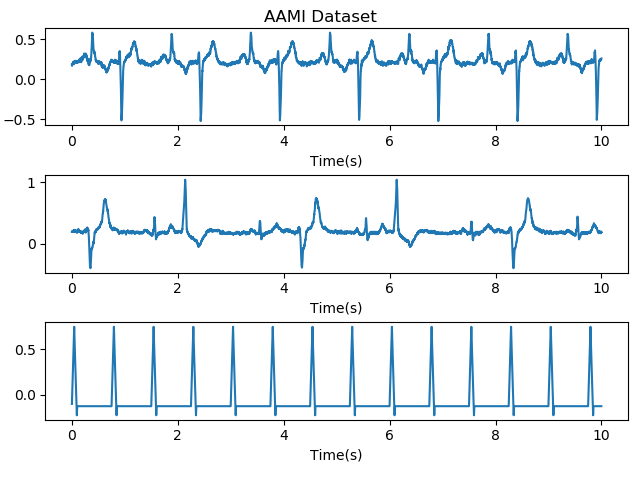
\includegraphics[width=\textwidth]{biosignals/aami_source.png}
    \caption{\en AAMI Dataset} \gr
    \label{fig:5.13}
\end{figure}
\noindent Τα σχήματα \en \ref{fig:5.14a} \gr και \en \ref{fig:5.14a} \gr είναι οι ανεξάρτητες συνιστώσες που εξάγει ο αλγόριθμος \en FastICA \gr για \en 'logcosh' \gr, τα σχήματα \en \ref{fig:5.15a} \gr   και \en \ref{fig:5.15b} \gr  για \en 'exp' \gr και τα σχήματα \en \ref{fig:5.16a} \gr και \en \ref{fig:5.16b} \gr για \en 'cube' \gr.
\begin{figure}[H]
    \centering
    \begin{subfigure}{0.48 \textwidth}
        \centering
       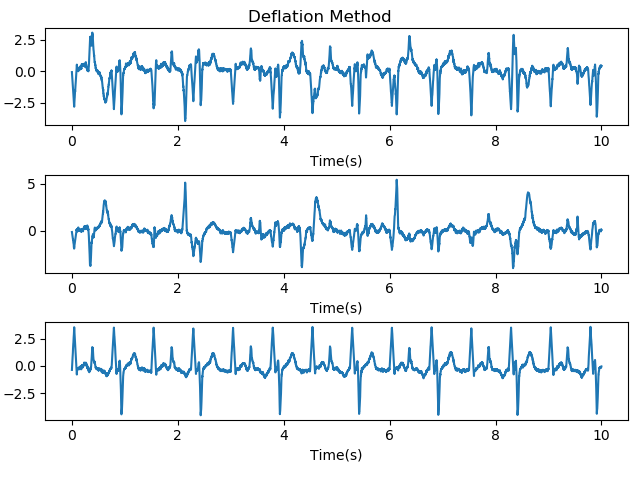
\includegraphics[width=\textwidth]{biosignals/aami_logcosh_def.png} \en
        \caption{Deflation} \gr
        \label{fig:5.14a}
    \end{subfigure}
    \hfill
    \begin{subfigure}{0.48 \textwidth}
        \centering
       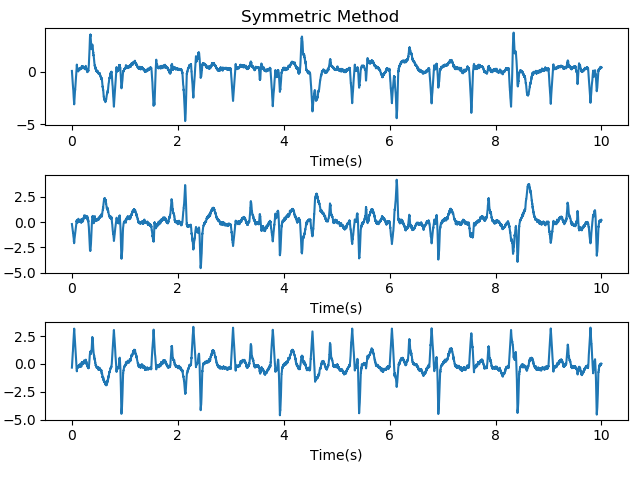
\includegraphics[width=\textwidth]{biosignals/aami_logcosh_sym.png} \en
        \en
        \caption{Symmetric} \gr
        \label{fig:5.14b}
    \end{subfigure}
    \gr
    \caption{Αποτελέσματα για \en g = 'logcosh' \gr}
\end{figure}
\begin{figure}[H]
    \centering
    \begin{subfigure}{0.48 \textwidth}
        \centering
       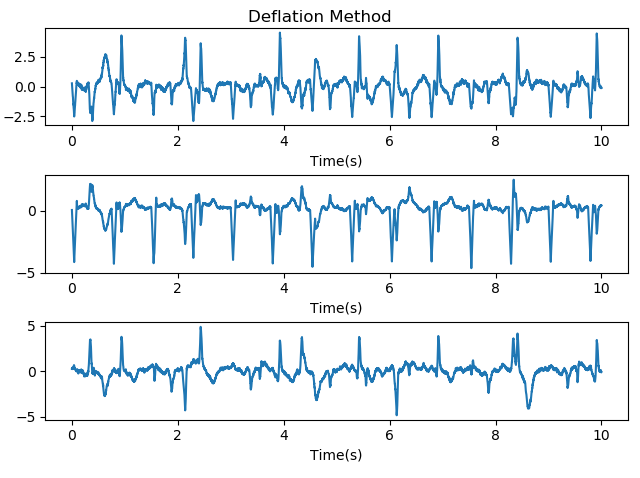
\includegraphics[width=\textwidth]{biosignals/aami_exp_def.png} \en
        \caption{Deflation} \gr
        \label{fig:5.15a}
    \end{subfigure}
    \hfill
    \begin{subfigure}{0.48 \textwidth}
        \centering
       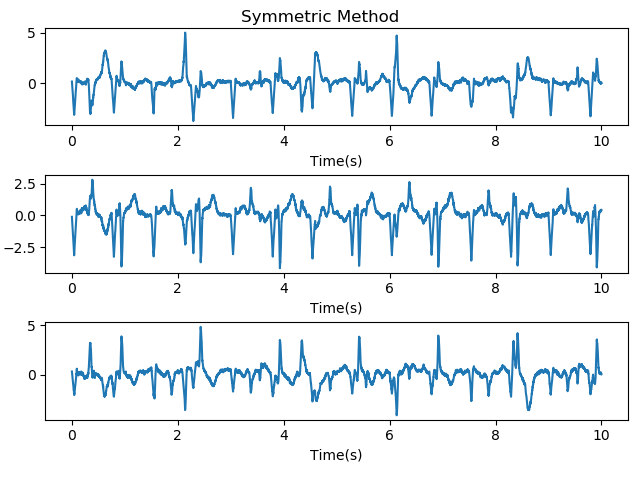
\includegraphics[width=\textwidth]{biosignals/aami_exp_sym.png} \en
        \en
        \caption{Symmetric} \gr
        \label{fig:5.15b}
    \end{subfigure}
    \gr
    \caption{Αποτελέσματα για \en g = 'exp' \gr}
\end{figure}
\begin{figure}[H]
    \centering
    \begin{subfigure}{0.48 \textwidth}
        \centering
       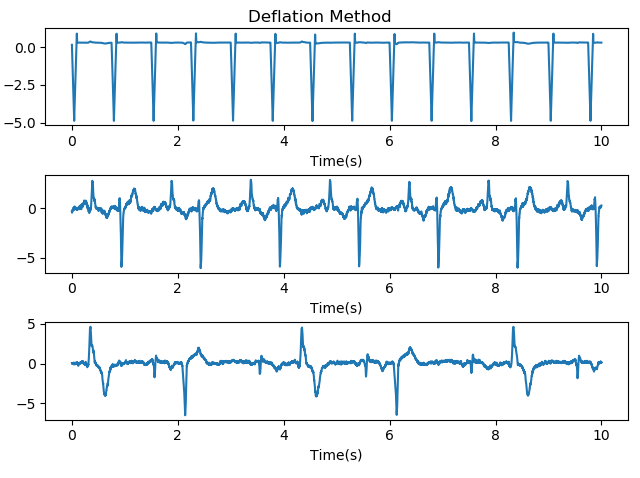
\includegraphics[width=\textwidth]{biosignals/aami_cube_def.png} \en
        \caption{Deflation} \gr
        \label{fig:5.16a}
    \end{subfigure}
    \hfill
    \begin{subfigure}{0.48 \textwidth}
        \centering
       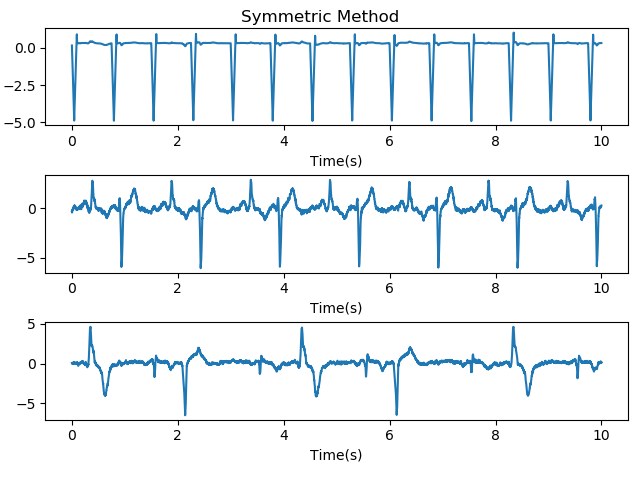
\includegraphics[width=\textwidth]{biosignals/aami_cube_sym.png} \en
        \en
        \caption{Symmetric} \gr
        \label{fig:5.16b}
    \end{subfigure}
    \gr
    \caption{Αποτελέσματα για \en g = 'cube' \gr}
\end{figure}
\noindent Στα σχήματα \en \ref{fig:5.17a} , \ref{fig:5.17b} \gr
φαίνονται οι περιοδικές συνιστώσες με τις αντίστοιχες περιόδους και στα σχήματα \en \ref{fig:5.18a}, \ref{fig:5.18b} \gr
τα αντίστοιχα περιοδικά σφάλματα.
\begin{figure}[H]
    \centering
    \begin{subfigure}{0.48 \textwidth}
        \centering
       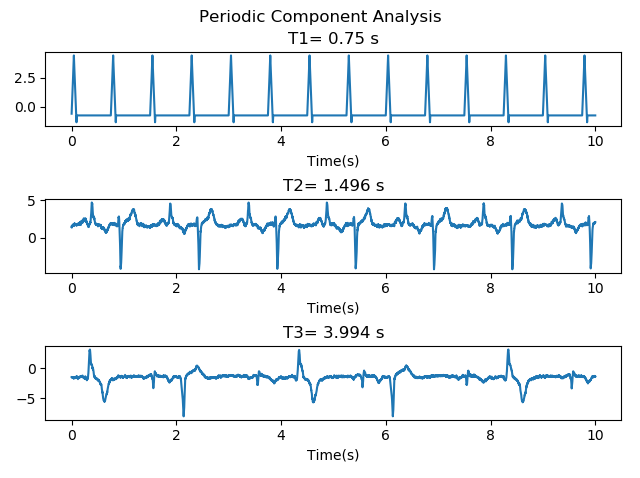
\includegraphics[width=\textwidth]{biosignals/aami_pica.png}\en
        \caption{\gr Κανονική \en \pi CA} \gr
        \label{fig:5.17a}
    \end{subfigure}
    \hfill
    \begin{subfigure}{0.48 \textwidth}
        \centering
       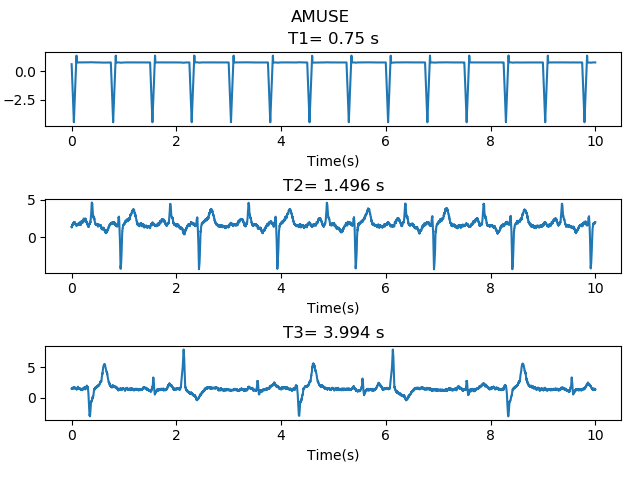
\includegraphics[width=\textwidth]{biosignals/aami_amuse.png}
        \en
        \caption{AMUSE} \gr
        \label{fig:5.17b}
    \end{subfigure}
    \gr
    \caption{Οι περιοδικές συνιστώσες του \en AAMI Dataset \gr για \en $T_1 = 0.75$ s, $T_2 = 1.496$ s \gr και \en $T_3 = 3.994$ s \gr }
\end{figure}
\begin{figure}[H]
    \centering
    \begin{subfigure}[b]{0.48 \textwidth}
        \centering
       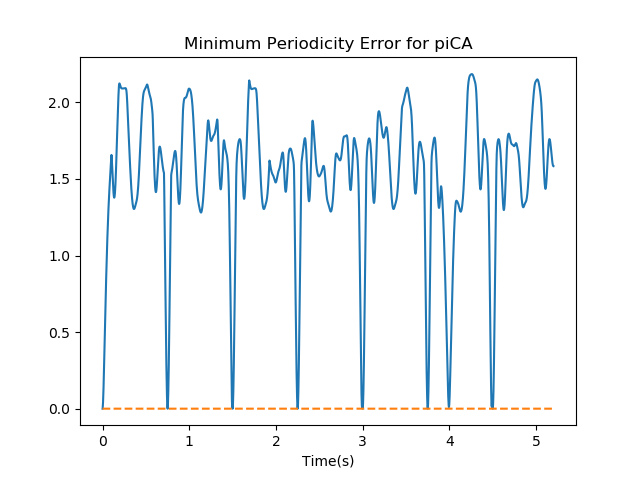
\includegraphics[width=\textwidth]{biosignals/aami_pica_error.png}\en
        \caption{\gr Κανονική \en \pi CA} \gr
        \label{fig:5.18a}
    \end{subfigure}
    \hfill
    \begin{subfigure}[b]{0.48 \textwidth}
        \centering
       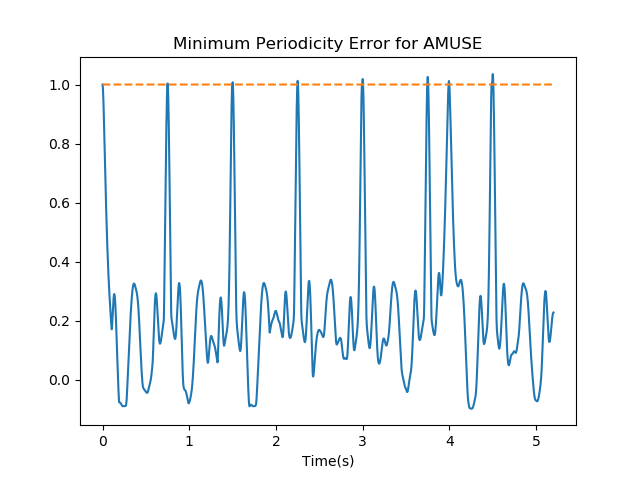
\includegraphics[width=\textwidth]{biosignals/aami_amuse_error.png}
        \en
        \caption{AMUSE} \gr
        \label{fig:5.18b}
    \end{subfigure}
    \gr
    \caption{Τα ελάχιστα περιοδικά σφάλματα για χρονική καθυστέρηση από 0 έως 5.2 δευτερόλεπτα}
\end{figure}
\noindent Βλέπουμε ότι ο αλγόριθμος π\en CA \gr βγάζει καθαρά τα σήματα όπως περιμέναμε, αναγνωρίζοντας και την περίοδο του καθενός. 'Οσο για τον αλγόριθμο \en Fast ICA, \gr στην περίπτωση \en 'cube' \gr λαμβάνουμε αρκετά καλά αποτελέσματα, δηλαδή μικρή αλλοίωση την τελική μορφή των σημάτων, και στις δυο προσεγγίσεις ενώ οι άλλες δύο περιπτώσεις αποτυγχάνουν πλήρως στην αναγνώριση των αρχικών σημάτων.  
\subsection{Πραγματικά Βιοσήματα - Παράδειγμα 1}
\justifying
Η βάση δεδομένων που θα χρησιμοποιήσουμε είναι η \en "Abdominal and Direct Fetal Electrocardiogram Database (adfecgdb)" \gr 
\cite{examples:20}\cite{examples:21}\cite{examples:22}
και συγκεκριμένα θα χρησιμοποιήσουμε τα σήματα \en r01.edf, \gr που κατεβάσαμε και αποθηκεύσαμε σε αρχείο \en .txt \gr μέσω του πακέτου \en WFDB \gr.
\\[0.5 \baselineskip]
Τα δεδομένα περιέχουν πολυκάναλες καταγραφές εμβρυακών ηλεκτροκαρδιογραφημάτων από 5 γυναίκες μεταξύ 38 και 41 εβδομάδων κύησης. Κάθε καταγραφή περιλαμβάνει 4 διαφορικά σήματα που αποκτήθηκαν από την κοιλία της μητέρας και 1 εμβρυακό ηλεκτροκαρδιογράφημα ως σήμα αναφοράς, από το κεφάλι του εμβρύου. Το εύρος ζώνης των σημάτων είναι \en 1 Hz - 150 Hz \gr και έχει φιλτραριστεί η παρεμβολή των \en 50 Hz \gr από την παροχή ρεύματος, όπως και οι χαμηλές συχνότητες του \en baseline drift \gr που οφείλονται στην κίνηση και την αναπνοή του μητέρας. Επιπλέον, όλα τα σήματα έχουν δειγματοληφθεί ταυτόχρονα με ρυθμό δειγματοληψίας \en $F_s = 1 kHz$ \gr με ακρίβεια 16 \en bits \gr και τα πλάτη των όλων των σημάτων είναι σε \en mV. \gr
\\ [0.5 \baselineskip]
Θα προσπαθήσουμε να εξάγουμε το μητρικό και το εμβρυακό \en ECG \gr με τις παραπάνω μεθόδους. Θα χρησιμοποιήσουμε το εμβρυακό ηλεκτροκαρδιογράφημα ως σήμα αναφοράς για την σύγκριση των εξαχθέντων συνιστωσών και τα υπόλοιπα ως μικτά σήματα προς εξαγωγή των συνιστωσών. Για την σύγκριση των σημάτων με το εμβρυακό \en ECG, \gr θα υπολογίσουμε τις θέσεις των \en RR-intervals, \gr δηλαδή της χρονικής διαφοράς μεταξύ \en R peaks \gr  από το σήμα αναφοράς. Σε όποια σήματα συμπίπτουν τα παραπάνω σημεία, θα αποτελούν εμβρυακά ενώ οποιοδήποτε περιοδικό σήμα, διάφορο του σήματος αναφοράς, θα αποτελεί μητρικό σήμα.
\\ [1.5 \baselineskip]
Στο σχήμα \ref{fig:5.19} φαίνονται τα πρώτα 12 δευτερόλεπτα του αρχείου \en r01 \gr και στο σχήμα \ref{fig:5.20} φαίνονται οι θέσεις των \en RR peaks \gr του εμβρυακού ηλεκτροκαρδιογραφήματος
\begin{figure}[H]
    \centering
    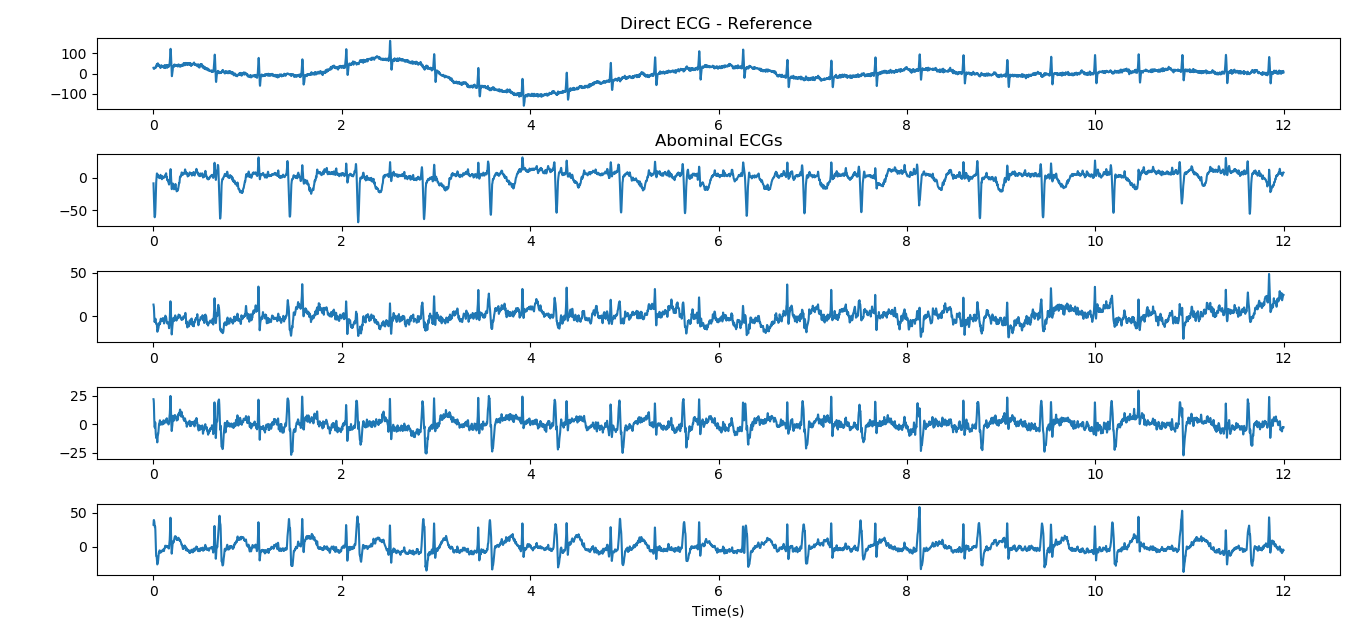
\includegraphics[width=\textwidth]{r01database/r01_12secs.png}
    \caption{Σήματα Ηλεκτροδίων της \en r01 \gr}
    \label{fig:5.19}
\end{figure}
\begin{figure}[H]
    \centering
    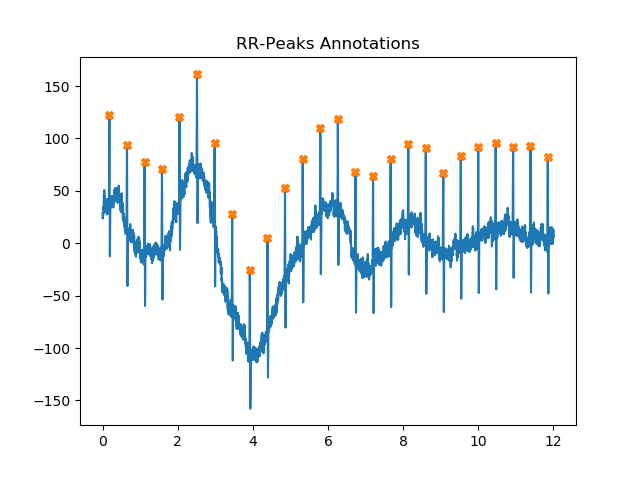
\includegraphics[width=0.7 \textwidth]{r01database/RR_peaks_annotations.png}
    \caption{Τα \en RR intervals \gr του εμβρυακού \en ECG \gr}
    \label{fig:5.20}
\end{figure}
\noindent Στα σχήματα \en \ref{fig:5.21a} \gr και \en \ref{fig:5.21b} \gr φαίνονται οι ανεξάρτητες συνιστώσες για \en 'logcosh'. \gr Στο πρώτο σχήμα, μπορούμε να πούμε ότι η 3η συνιστώσα αποτελεί το εμβρυακό και η 4η το μητρικό ενώ στο δεύτερο σχήμα, το 1ο είναι το εμβρυακό και το 4ο το μητρικό. Η Συμμετρική προσέγγιση βλέπουμε ότι αναγνωρίζει καλύτερα το εμβρυακό σήμα ενώ για το μητρικό δεν μπορούμε να αποφανθούμε περαιτέρω.
\begin{figure}[H]
    \centering
    \begin{subfigure}{0.48 \textwidth}
        \centering
       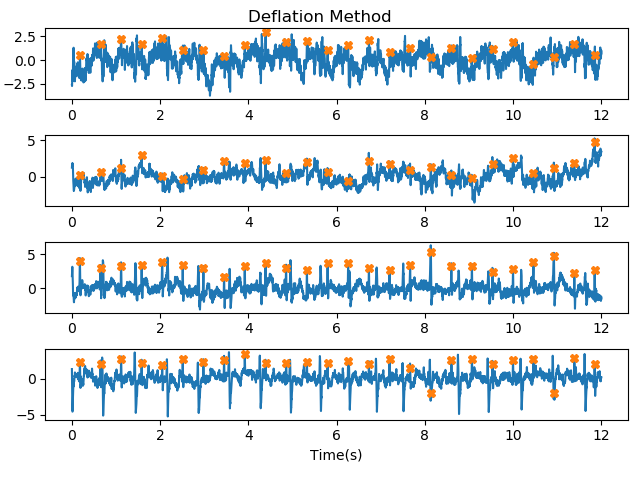
\includegraphics[width=\textwidth]{r01database/logcosh_def.png} \en
        \caption{Deflation} \gr
        \label{fig:5.21a}
    \end{subfigure}
    \hfill
    \begin{subfigure}{0.48 \textwidth}
        \centering
       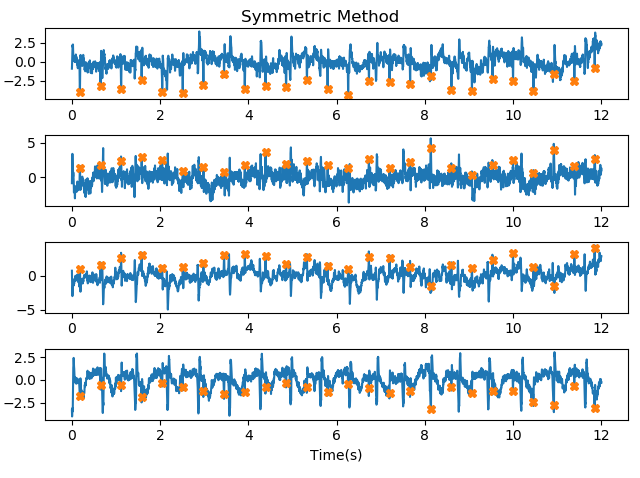
\includegraphics[width=\textwidth]{r01database/logcosh_sym.png} \en
        \en
        \caption{Symmetric} \gr
        \label{fig:5.21b}
    \end{subfigure}
    \gr
    \caption{Αποτελέσματα για \en g = 'logcosh' \gr}
\end{figure}
%%
\noindent Στα σχήματα \en \ref{fig:5.22a} \gr και \en \ref{fig:5.22b} \gr φαίνονται οι ανεξάρτητες συνιστώσες για \en 'exp'. \gr Στο πρώτο σχήμα, η 4η συνιστώσα είναι πιο κοντά στο εμβρυακό \en ECG \gr ενώ στπ δεύτερο σχήμα, το 1ο είναι το εμβρυακό και το 4ο το μητρικό. Όπως και στην \en 'logcosh' \gr περίπτωση, βλέπουμε ότι η Συμμετρική προσέγγιση παράγει καλύτερα αποτελέσματα.
\begin{figure}[H]
    \centering
    \begin{subfigure}{0.48 \textwidth}
        \centering
       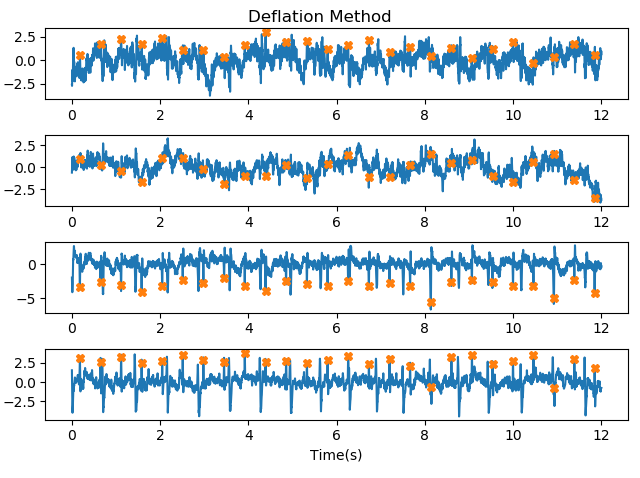
\includegraphics[width=\textwidth]{r01database/exp_def.png} \en
        \caption{Deflation} \gr
        \label{fig:5.22a}
    \end{subfigure}
    \hfill
    \begin{subfigure}{0.48 \textwidth}
        \centering
       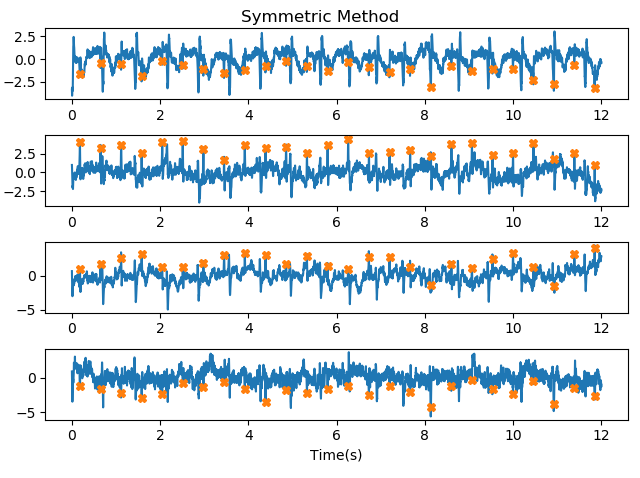
\includegraphics[width=\textwidth]{r01database/exp_sym.png} \en
        \en
        \caption{Symmetric} \gr
        \label{fig:5.22b}
    \end{subfigure}
    \gr
    \caption{Αποτελέσματα για \en g = 'exp' \gr}
\end{figure}
\noindent Στα σχήματα \en \ref{fig:5.23a} \gr και \en \ref{fig:5.23b} \gr φαίνονται οι ανεξάρτητες συνιστώσες για \en 'cube'. \gr Στο πρώτο σχήμα, η 1η συνιστώσα είναι το εμβρυακό \en ECG \gr και το 2ο το μητρικό ενώ στο δεύτερο σχήμα, το 4ο είναι το εμβρυακό και το 2ο το μητρικό. Σε αντίθεση με τις άλλες συναρτήσεις, η συνάρτηση \en 'cube' \gr εξάγει καλά αποτελέσματα και στις δύο περιπτώσεις.
\begin{figure}[H]
    \centering
    \begin{subfigure}{0.48 \textwidth}
        \centering
       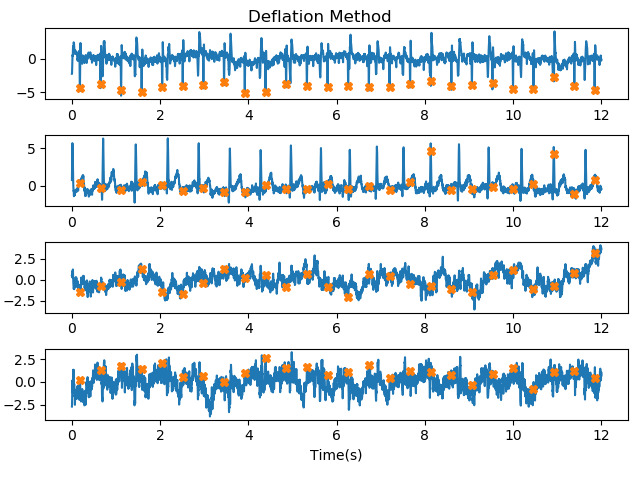
\includegraphics[width=\textwidth]{r01database/cube_def.png} \en
        \caption{Deflation} \gr
        \label{fig:5.23a}
    \end{subfigure}
    \hfill
    \begin{subfigure}{0.48 \textwidth}
        \centering
       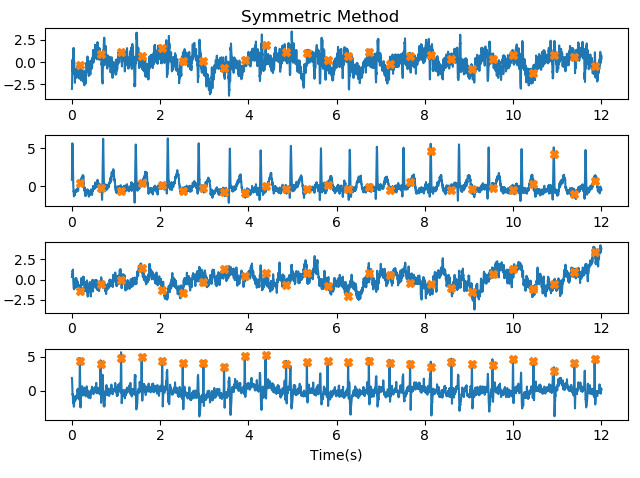
\includegraphics[width=\textwidth]{r01database/cube_sym.png} \en
        \en
        \caption{Symmetric} \gr
        \label{fig:5.23b}
    \end{subfigure}
    \gr
    \caption{Αποτελέσματα για \en g = 'cube' \gr}
\end{figure}
%
\noindent Στο σχήμα \ref{fig:5.24} φαίνονται οι περιοδικές συνιστώσες που εξάγονται από τον π\en CA. \gr Το πρώτο σχήμα δίνει ως πρώτη συνιστώσα το εμβρυακό \en ECG \gr και το δεύτερο σχήμα το μητρικό αντίστοιχα. Πρέπει να τονίσουμε ότι στο δεύτερο σχήμα, πήραμε ως αναφορά τα \en R peaks \en του μητρικού \en ECG \gr. Παρατηρούμε επίσης ότι η 3η συνιστώσα του πρώτου σχήματος και του δεύτερου σχήματος είναι το μητρικό και εμβρυακό \en ECG \gr αντίστοιχα.
\begin{figure}[H] 
    \centering
    \begin{subfigure}{0.48 \textwidth}
        \centering
        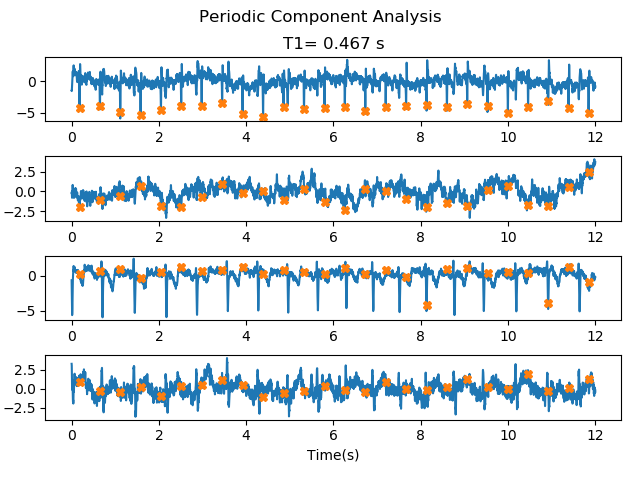
\includegraphics[width=\textwidth]{r01database/infant_pica.png}\en
    \end{subfigure}
    \hfill
    \begin{subfigure}{0.48 \textwidth}
        \centering
        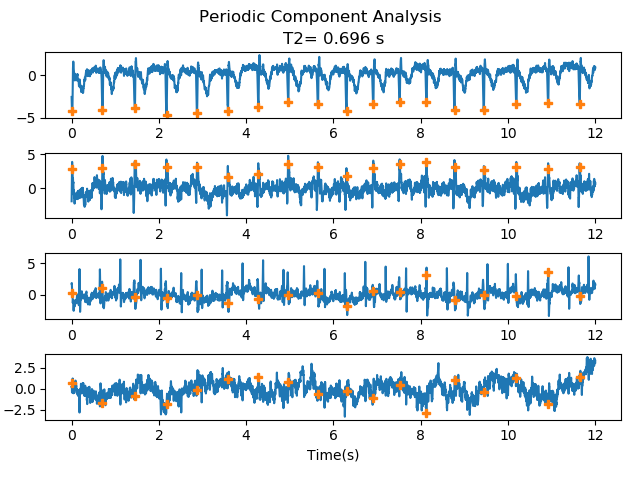
\includegraphics[width=\textwidth]{r01database/mother_pica.png}\en
    \end{subfigure}
    \gr
    \caption{Περιοδικές συνιστώσες για π\en CA \gr με περιόδους \en $Τ_1 = 0.467 s$ \gr και \en $Τ_2 = 0.696 s$ \gr  }
    \label{fig:5.24}
\end{figure} 
%
\noindent Στο σχήμα \ref{fig:5.25} φαίνονται οι περιοδικές συνιστώσες που εξάγονται μέσω \en AMUSE. \gr Παρατηρούμε τα ίδια ακριβώς αποτελέσματα με τον αλγόριθμο π\en CA. \gr
\begin{figure}[H] 
    \centering
    \begin{subfigure}{0.48 \textwidth}
        \centering
        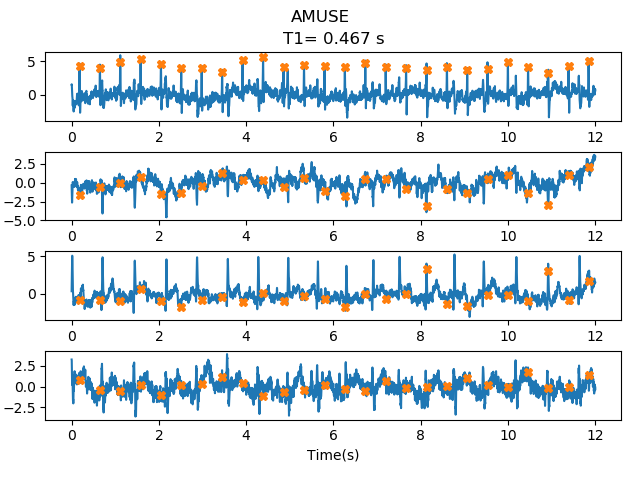
\includegraphics[width=\textwidth]{r01database/amuse_infant.png}\en
    \end{subfigure}
    \hfill
    \begin{subfigure}{0.48 \textwidth}
        \centering
        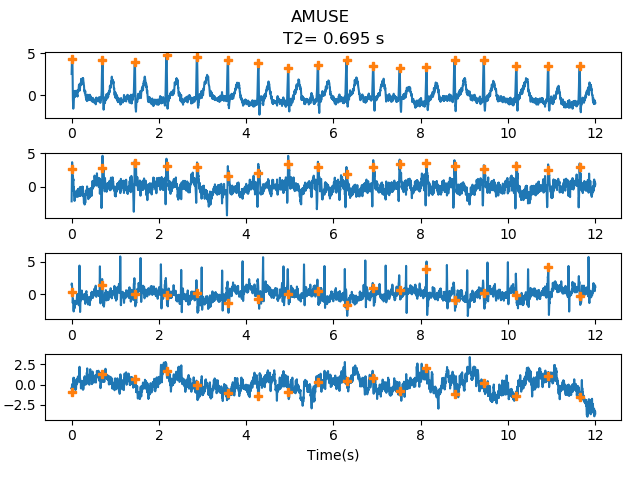
\includegraphics[width=\textwidth]{r01database/amuse_mother.png}\en
    \end{subfigure}
    \gr
    \caption{Περιοδικές συνιστώσες για \en AMUSE \gr με περιόδους \en $Τ_1 = 0.467 s$ \gr και \en $Τ_2 = 0.696 s$ \gr  }
    \label{fig:5.25}
\end{figure} 
\noindent Τέλος, στο σχήμα φαίνονται τα περιοδικά σφάλματα για τους αλγόριθμους π\en CA \gr και \en AMUSE. \gr
\begin{figure}[H]
    \centering
    \begin{subfigure}[b]{0.48 \textwidth}
        \centering
       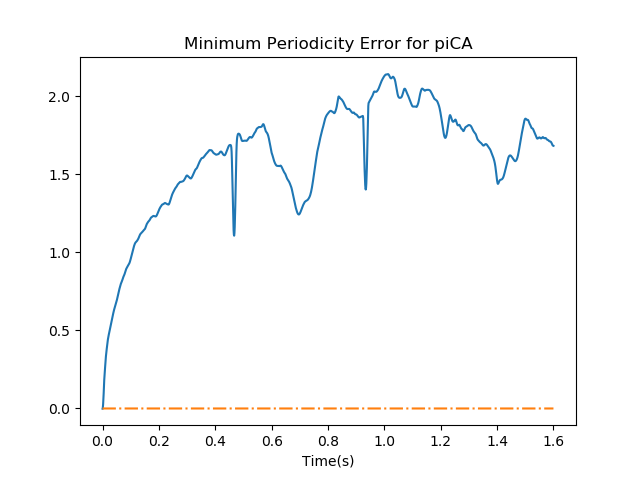
\includegraphics[width=\textwidth]{r01database/pica_error.png}\en
        \caption{\gr Κανονική \en \pi CA} \gr
    \end{subfigure}
    \hfill
    \begin{subfigure}[b]{0.48 \textwidth}
        \centering
        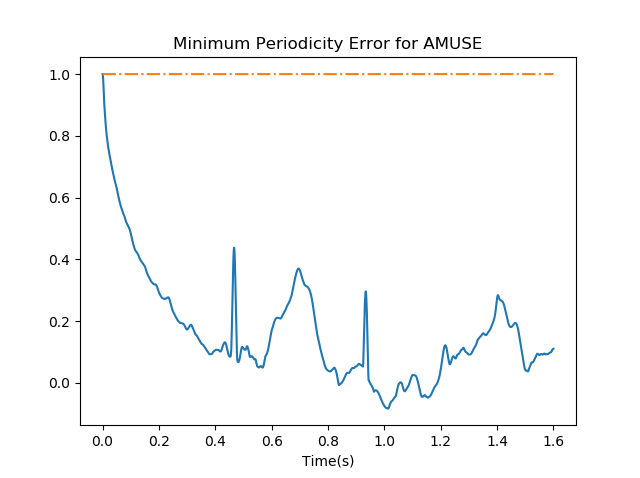
\includegraphics[width=\textwidth]{r01database/amuse_error.png}\en
        \caption{AMUSE} \gr
    \end{subfigure}
    \gr
    \caption{Τα ελάχιστα περιοδικά σφάλματα για χρονική καθυστέρηση από 0 έως 1.6 δευτερόλεπτα}
    \label{fig:5.26}
\end{figure}
\subsection{Πραγματικά Βιοσήματα - Περίπτωση 2}
\justifying
Η βάση δεδομένων που θα χρησιμοποιήσουμε είναι η \en DaISy \gr \cite{daisy:24} που περιέχει πολυκάναλες καταγραφές του δερματικού δυναμικού μιας εγκύου γυναίκας. Τα δεδομένα περιέχουν 5 καταγραφές γύρω από την κοιλιακή κοιλότητα της μητέρας και 3 θωρακικές καταγραφές που φαίνονται στο σχήμα \ref{fig:5.27}. Τα σήματα έχουν δειγματοληφθεί ταυτόχρονα με ρυθμό δειγματοληψίας 250 \en Hz \gr, έχουν διάρκεια 10 δευτερολέπτων και το πλάτος τους είναι σε \en mV. \gr Τα σήματα είναι σε μορφή \en .dat \gr με πρώτη στήλη τα δείγματα σε μορφή δευτερολέπτων ενώ οι υπόλοιπες στήλες τις παρατηρήσεις των ηλεκτροκαρδιογραφημάτων. 
% butterworth filtro
\newpage
\noindent Ο σκοπός μας είναι, όπως και στην προηγούμενη ενότητα, να αναγνωρίσουμε το εμβρυακό και το μητρικό \en ECG \gr με μόνη διαφορά ότι το σήμα αναφοράς θα είναι ένα από τα θωρακικά ηλεκτροκαρδιογραφήματα των δεδομένων, συγκεκριμένα το μητρικό \en ECG. \gr Άρα, οποιοδήποτε περιοδικό σήμα με διαφορετικά \en R peaks \gr θα είναι το εμβρυακό.
\begin{figure}[H]
    \centering
    \begin{subfigure}[b]{0.48 \textwidth}
        \centering
       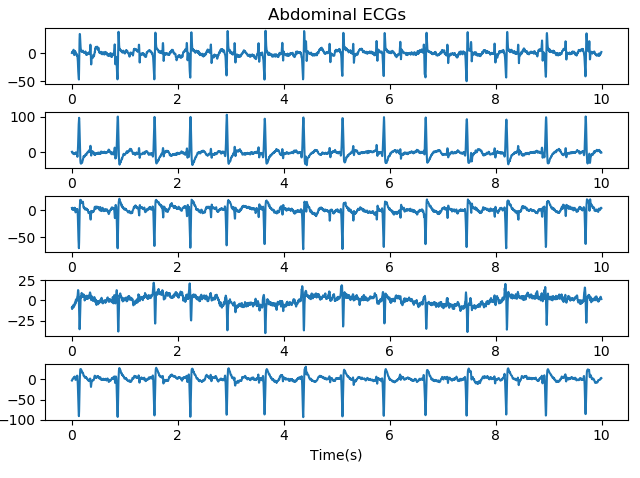
\includegraphics[width=\textwidth]{daisy/Abdominals.png}\en
        \caption{\gr Κοιλιακά Ηλεκτροκαρδιογραφήματα} \gr
    \end{subfigure}
    \hfill
    \begin{subfigure}[b]{0.48 \textwidth}
        \centering
        \includegraphics[width=\textwidth]{daisy/Thoracic.png}\en
        \caption{\gr Θωρακικά Ηλεκτροκαρδιογραφήματα} \gr
    \end{subfigure}
    \gr
    \caption{Βάση δεδομένων \en DaISy \gr}
    \label{fig:5.27}
\end{figure}
\begin{figure}[H]
    \centering
    \includegraphics[width=0.7 \textwidth]{daisy/maternal_reference.png}
    \caption{Τα \en RR intervals \gr του μητρικού \en ECG \gr που λαμβάνονται από τον θώρακα}
    \label{fig:5.28}
\end{figure}
\noindent Αξίζει να σημειωθεί ότι η εφαρμογή φίλτρου δεν φέρει μεγάλο αποτέλεσμα,καθώς όπως φαίνεται και από το σχήμα \ref{fig:5.35}, το φάσμα των παρατηρήσεων είναι γύρω από τις συχνότητες \en 1 Hz  \gr έως \en 20Hz. \gr Οπότε καλούμαστε να εξάγουμε τις συνιστώσες ενδιαφέροντος υπό την παρουσία θορύβου.
\begin{figure}[H]
    \centering
    \includegraphics[width=0.7 \textwidth]{daisy/fft.png}
    \caption{Συχνοτικό φάσμα των παρατηρήσεων}
    \label{fig:5.35}
\end{figure}
\noindent Στα σχήματα \ref{fig:5.29a} και \ref{fig:5.29b} φαίνονται οι ανεξάρτητες συνιστώσες για \en 'logcosh' \gr. Παρατηρούμε ότι στην πρώτη εικόνα, τα σχήματα 7,8 αντιστοιχούν στο μητρικό \en ECG \gr ενώ το 6 θυμίζει το εμβρυακό, ενώ στην δεύτερη εικόνα δεν μπορούμε να βγάλουμε συμπεράσματα. 
\begin{figure}[H]
    \centering
    \begin{subfigure}{0.48 \textwidth}
        \centering
       \includegraphics[width=\textwidth]{daisy/logcosh_def.png} \en
        \caption{Deflation} \gr
        \label{fig:5.29a}
    \end{subfigure}
    \hfill
    \begin{subfigure}{0.48 \textwidth}
        \centering
       \includegraphics[width=\textwidth]{daisy/logcosh_sym.png} \en
        \en
        \caption{Symmetric} \gr
        \label{fig:5.29b}
    \end{subfigure}
    \gr
    \caption{Αποτελέσματα για \en g = 'logcosh' \gr}
\end{figure}
\noindent Στα σχήματα \ref{fig:5.30a} και \ref{fig:5.30b} φαίνονται οι ανεξάρτητες συνιστώσες για \en 'exp' \gr. Παρατηρούμε ότι στην πρώτη εικόνα, το σχήμα 8 αντιστοιχεί στο μητρικό \en ECG \gr χωρίς να έχουμε βρει το εμβρυακό ενώ στην δεύτερη εικόνα δεν μπορούμε πάλι να βγάλουμε συμπεράσματα. 
\begin{figure}[H]
    \centering
    \begin{subfigure}{0.48 \textwidth}
        \centering
       \includegraphics[width=\textwidth]{daisy/exp_def.png} \en
        \caption{Deflation} \gr
        \label{fig:5.30a}
    \end{subfigure}
    \hfill
    \begin{subfigure}{0.48 \textwidth}
        \centering
       \includegraphics[width=\textwidth]{daisy/exp_sym.png} \en
        \en
        \caption{Symmetric} \gr
        \label{fig:5.30b}
    \end{subfigure}
    \gr
    \caption{Αποτελέσματα για \en g = 'exp' \gr}
\end{figure}
\noindent Στα σχήματα \ref{fig:5.31a} και \ref{fig:5.31b} φαίνονται οι ανεξάρτητες συνιστώσες για \en 'cube' \gr. Παρατηρούμε ότι στην πρώτη εικόνα, τα σχήματα 1, 2 και 3 αντιστοιχούν στο μητρικό \en ECG \gr και το 4ο στο εμβρυακό, ενώ στην συμμετρική προσέγγιση, το 4ο σχήμα είναι το εμβρυακό και τα σχήματα 1, 3 και 5 το μητρικό. Βλέπουμε επιπλέον ότι ο αλγόριθμος \en FastICA \gr δίνει αρκετά καλά αποτελέσματα με την χρήση της συνάρτησης \en $x^3$ \gr.
\begin{figure}[H]
    \centering
    \begin{subfigure}{0.48 \textwidth}
        \centering
       \includegraphics[width=\textwidth]{daisy/cube_def.png} \en
        \caption{Deflation} \gr
        \label{fig:5.31a}
    \end{subfigure}
    \hfill
    \begin{subfigure}{0.48 \textwidth}
        \centering
       \includegraphics[width=\textwidth]{daisy/cube_sym.png} \en
        \en
        \caption{Symmetric} \gr
        \label{fig:5.31b}
    \end{subfigure}
    \gr
    \caption{Αποτελέσματα για \en g = 'cube' \gr}
\end{figure}
\noindent Στο σχήμα \ref{fig:5.32} φαίνονται οι περιοδικές συνιστώσες που εξάγονται από τον π\en CA. Η πρώτη γραφική παράσταση φανερώνει ως πρώτη συνιστώσα το εμβρυακό ηλεκτροκαρδιογράφημα με την αντίστοιχη περίοδο ενώ στο τέλος βλέπουμε το μητρικό. Αντίστοιχα, στην δεύτερη γραφική παράσταση, παρατηρούμε ότι το μητρικό ηλεκτροκαρδιογράφημα φαίνεται στην πρώτη θέση με την παρουσία θορύβου, όσο αφορά τα \en R peaks, \gr αλλά και στην πέμπτη καθαρότερα, ακολουθώντας τα εμβρυακά. Αυτό το γεγονός μάλλον οφείλεται στην παρουσία θορύβου, όπως αναφέραμε παραπάνω, αλλά κα στην ακρίβεια του βήματος που χρησιμοποιούμε ως \en timelag \gr.
\begin{figure}[H] 
    \centering
    \begin{subfigure}{0.48 \textwidth}
        \centering
        \includegraphics[width=\textwidth]{daisy/pica_infant.png}\en
    \end{subfigure}
    \hfill
    \begin{subfigure}{0.48 \textwidth}
        \centering
        \includegraphics[width=\textwidth]{daisy/pica_maternal.png}
        \en
    \end{subfigure}
    \gr
    \caption{Περιοδικές συνιστώσες για π\en CA \gr με περιόδους \en $Τ_1 = 0.448 s$ \gr και \en $Τ_2 = 0.74 s$ \gr  }
    \label{fig:5.32}
\end{figure} 
\noindent Αντίστοιχα, στο σχήμα \ref{fig:5.33} φαίνονται οι περιοδικές συνιστώσες που εξάγoνται από τον \en AMUSE. \gr Βλέπουμε τα ίδια ακριβώς ίδια αποτελέσματα με τον π\en CA \gr. 
\begin{figure}[H] 
    \centering
    \begin{subfigure}{0.48 \textwidth}
        \centering
        \includegraphics[width=\textwidth]{daisy/amuse_infant.png}\en
    \end{subfigure}
    \hfill
    \begin{subfigure}{0.48 \textwidth}
        \centering
        \includegraphics[width=\textwidth]{daisy/amuse_maternal.png}
        \en
    \end{subfigure}
    \gr
    \caption{Περιοδικές συνιστώσες για \en AMUSE \gr με περιόδους \en $Τ_1 = 0.448 s$ \gr και \en $Τ_2 = 0.74 s$ \gr  }
    \label{fig:5.33}
\end{figure} 
\noindent Τέλος, στο σχήμα \ref{fig:5.34} φαίνονται τα περιοδικά σφάλματα για τους παραπάνω αλγορίθμους.
\begin{figure}[H]
    \centering
    \begin{subfigure}[b]{0.48 \textwidth}
        \centering
       \includegraphics[width=\textwidth]{daisy/pica_error.png}\en
        \caption{\gr Κανονική \en \pi CA} \gr
    \end{subfigure}
    \hfill
    \begin{subfigure}[b]{0.48 \textwidth}
        \centering
        \includegraphics[width=\textwidth]{daisy/amuse_error.png}\en
        \caption{AMUSE} \gr
    \end{subfigure}
    \gr
    \caption{Τα ελάχιστα περιοδικά σφάλματα για χρονική καθυστέρηση από 0 έως 1.2 δευτερόλεπτα}
    \label{fig:5.34}
\end{figure}
\noindent Όπως και με τα προηγούμενα σήματα, βλέπουμε ότι οι αλγόριθμοι π\en CA \gr και \en AMUSE \gr αναγνωρίζουν αρκετά καλά τα σήματα ενδιαφέροντος, σε αντίθεση με τον αλγόριθμο \en FastICA. \gr
\subsection{Αξιολόγηση στην εξαγωγή βιοσημάτων}
\justifying
Για την αξιολόγηση των πραγματικών σημάτων \cite{criterion:25}, θα υπολογίσουμε την ακρίβεια - \en Accuracy \gr και την ευαισθησία - \en Sensivity \gr στα αποτελέσματα που λάβαμε από τον π\en CA \gr στα κεφάλαια 5.2.2 και 5.2.3 . Εφόσον με τον αλγόριθμο π\en CA \gr λαμβάνουμε την περιοδική συνιστώσα με ελάχιστο περιοδικό σφάλμα σε κάθε \en timelag, \gr αρκεί μόνο να εξετάσουμε την πρώτη συνιστώσα για κάθε περίοδο.
\\[0.5 \baselineskip]
Ως \en Sensivity \gr ορίζεται το ποσοστό των \en R peaks \gr που αναγνωρίστηκαν σωστά από τον αλγόριθμο και ως \en Accuracy \gr την συνολική ορθότητα της μεθόδου. Συγκεκριμένα:
\begin{align} \label{eq:5.2.1}
    Sensivity = \frac{TP}{TP+FN} 
\end{align}
\begin{align} \label{eq:5.2.2}
    Accuracy = \frac{TP}{TP+FN+FP}
\end{align}
όπου
\begin{itemize}
    \item \en TP (True Positive) \gr ο αριθμός των \en peak \gr του εκάστοτε σήματος αναφοράς
    \item \en FN (False Negative) \gr ο αριθμός των \en peak \gr που παρέλειψε να αναγνωρίσει ο αλγόριθμος
    \item \en FP (False Positive) \gr ο αριθμός των \en peak \gr που αναγνώρισε εσφαλμένα ο αλγόριθμος
\end{itemize}
Στους παρακάτω πίνακες φαίνονται τα ποσοστά των κριτηρίων των σχέσεων \eqref{eq:5.2.1} και \eqref{eq:5.2.2}:
\begin{table}[H] 
\centering
\begin{tabular}{|c|c|c|} 
\hline
          & \gr Εμβρυακό \en ECG  & \gr Μητρικό \en ECG  \\ \hline
\en Sensivity & 100 \% &  100 \% \\ \hline
\en Accuracy  & 100 \% &  100 \% \\ \hline
\end{tabular}
\gr
\caption{Απόδοση του \en abfecg dataset\gr }
\label{table:5.3}
\end{table}
\begin{table}[H] 
\centering
\begin{tabular}{|c|c|c|} 
\hline
          & \gr Εμβρυακό \en ECG  & \gr Μητρικό \en ECG  \\ \hline
\en Sensivity & 100 \% &  100 \% \\ \hline
\en Accuracy  & 100 \% &  87.5 \% \\ \hline
\end{tabular}
\gr
\caption{Απόδοση του \en DaISy dataset\gr }
\label{table:5.4}
\end{table}
\noindent Στo \en abfecgdb dataset \gr έχουμε 26 κορυφές για το εμβρυακό \en ECG \gr και 18 κορυφές για το μητρικό, με τον αλγόριθμο να τις αναγνωρίζει όλες. Απο την άλλη, στο \en DaISy dataset, \gr έχουμε 26 κορυφές για το εμβρυακό, που αναγνωρίζονται όλες και 14 για το μητρικό, εκ των οποίων οι 2 αναγνωρίζονται εσφαλμένα.